\documentclass[tikz,border=6pt]{standalone}
\usepackage{amsmath}
\usetikzlibrary{arrows.meta,positioning,calc,chains}
\begin{document}
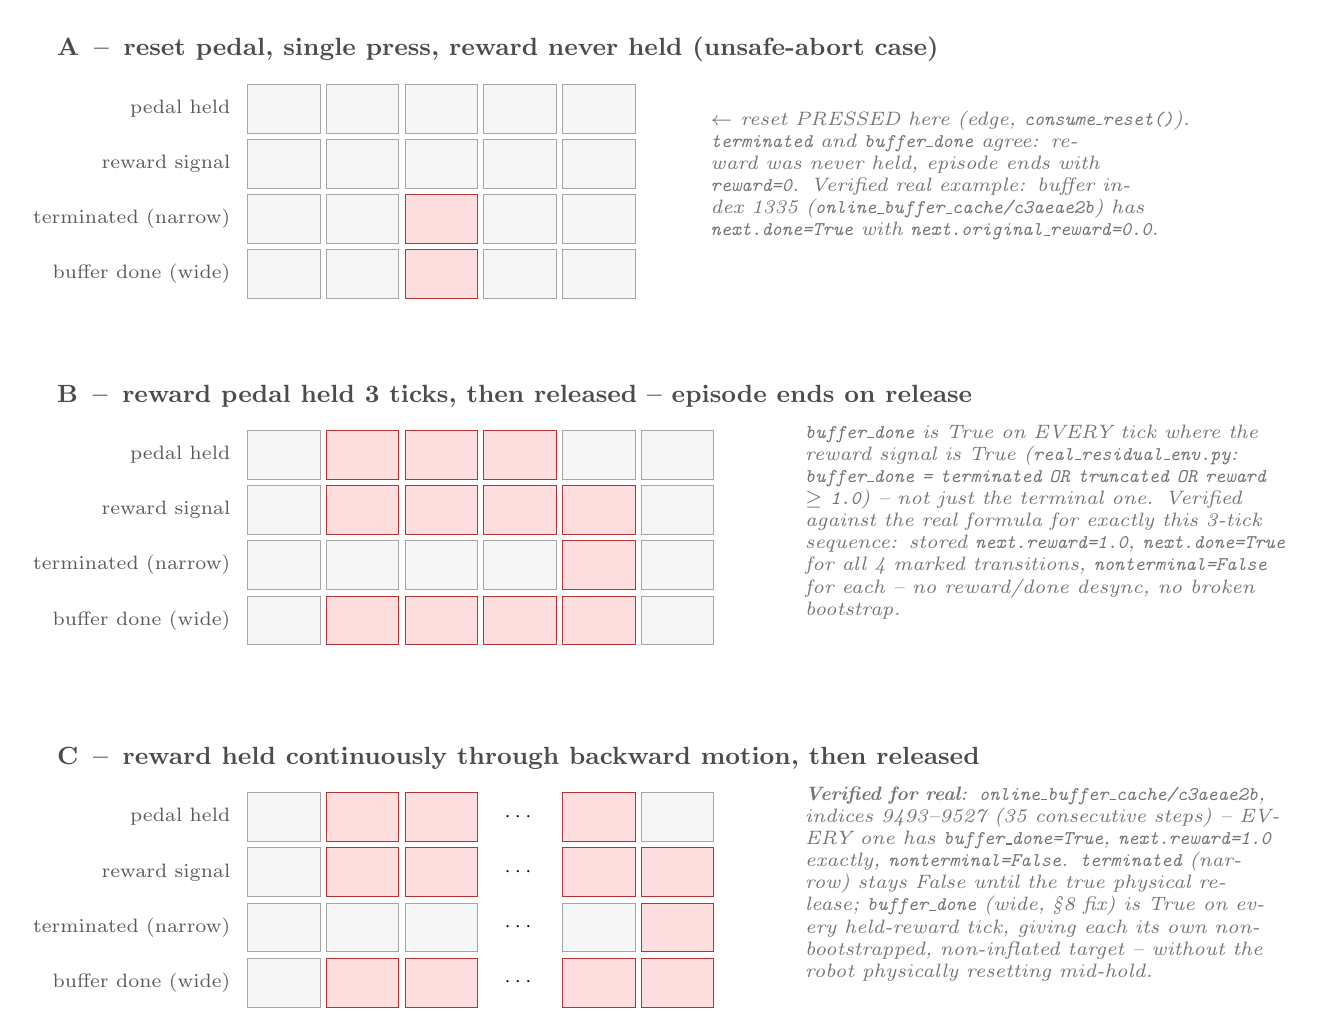
\begin{tikzpicture}[
    >={Latex[length=2.2mm,width=1.6mm]}, font=\small,
    cell/.style={draw,very thin,align=center,minimum width=0.92cm,minimum height=0.62cm,inner sep=0pt,font=\scriptsize},
    T/.style={cell,fill=truefill,draw=trueline},
    F/.style={cell,fill=falsefill,draw=black!35},
    rowlbl/.style={font=\scriptsize,anchor=east,text=black!65,inner sep=2pt},
    scen/.style={font=\small\bfseries,text=black!70,anchor=west},
    note/.style={font=\scriptsize\itshape,align=left,text=black!55,text width=6.2cm,anchor=west},
]
\definecolor{trueline}{RGB}{178,52,52}    \definecolor{truefill}{RGB}{253,222,222}
\definecolor{falsefill}{RGB}{246,246,246}
\definecolor{bufline}{RGB}{170,108,20}

% Column x-positions start at 1.7 (leaves room for the row labels, which end at x=1.5)
\def\gx{3.0}

% ================= Scenario A: reset press with no reward held (unsafe abort) =================
\node[scen] at (0,10.6) {A \,--\, reset pedal, single press, reward never held (unsafe-abort case)};
\node[rowlbl] at (2.4,10.6-0.75) {pedal held};
\node[rowlbl] at (2.4,10.6-1.45) {reward signal};
\node[rowlbl] at (2.4,10.6-2.15) {terminated (narrow)};
\node[rowlbl] at (2.4,10.6-2.85) {buffer done (wide)};
\foreach \v [count=\i from 0] in {F,F,F,F,F} { \node[\v] at (\gx+\i*1.0,10.6-0.75) {}; }
\foreach \v [count=\i from 0] in {F,F,F,F,F} { \node[\v] at (\gx+\i*1.0,10.6-1.45) {}; }
\foreach \v [count=\i from 0] in {F,F,T,F,F} { \node[\v] at (\gx+\i*1.0,10.6-2.15) {}; }
\foreach \v [count=\i from 0] in {F,F,T,F,F} { \node[\v] at (\gx+\i*1.0,10.6-2.85) {}; }
\node[note] at (\gx+5.3,10.6-1.6) {$\leftarrow$ reset PRESSED here (edge, \texttt{consume\_reset()}). \texttt{terminated} and \texttt{buffer\_done} agree: reward was never held, episode ends with \texttt{reward=0}. Verified real example: buffer index 1335 (\texttt{online\_buffer\_cache/c3aeae2b}) has \texttt{next.done=True} with \texttt{next.original\_reward=0.0}.};

% ================= Scenario B: reward hold then release (short) =================
\node[scen] at (0,6.2) {B \,--\, reward pedal held 3 ticks, then released -- episode ends on release};
\node[rowlbl] at (2.4,6.2-0.75) {pedal held};
\node[rowlbl] at (2.4,6.2-1.45) {reward signal};
\node[rowlbl] at (2.4,6.2-2.15) {terminated (narrow)};
\node[rowlbl] at (2.4,6.2-2.85) {buffer done (wide)};
\foreach \v [count=\i from 0] in {F,T,T,T,F,F} { \node[\v] at (\gx+\i*1.0,6.2-0.75) {}; }
\foreach \v [count=\i from 0] in {F,T,T,T,T,F} { \node[\v] at (\gx+\i*1.0,6.2-1.45) {}; }
\foreach \v [count=\i from 0] in {F,F,F,F,T,F} { \node[\v] at (\gx+\i*1.0,6.2-2.15) {}; }
\foreach \v [count=\i from 0] in {F,T,T,T,T,F} { \node[\v] at (\gx+\i*1.0,6.2-2.85) {}; }
\node[note] at (\gx+6.5,6.2-1.6) {\texttt{buffer\_done} is True on EVERY tick where the reward signal is True (\texttt{real\_residual\_env.py}: \texttt{buffer\_done = terminated OR truncated OR reward} $\geq$ \texttt{1.0}) -- not just the terminal one. Verified against the real formula for exactly this 3-tick sequence: stored \texttt{next.reward=1.0}, \texttt{next.done=True} for all 4 marked transitions, \texttt{nonterminal=False} for each -- no reward/done desync, no broken bootstrap.};

% ================= Scenario C: reward held through extra (non-rewarding) motion =================
\node[scen] at (0,1.6) {C \,--\, reward held continuously through backward motion, then released};
\node[rowlbl] at (2.4,1.6-0.75) {pedal held};
\node[rowlbl] at (2.4,1.6-1.45) {reward signal};
\node[rowlbl] at (2.4,1.6-2.15) {terminated (narrow)};
\node[rowlbl] at (2.4,1.6-2.85) {buffer done (wide)};
\node[F] at (\gx+0,1.6-0.75) {}; \node[T] at (\gx+1,1.6-0.75) {}; \node[T] at (\gx+2,1.6-0.75) {};
\node[cell,fill=white,draw=none] at (\gx+3,1.6-0.75) {$\cdots$}; \node[T] at (\gx+4,1.6-0.75) {}; \node[F] at (\gx+5,1.6-0.75) {};
\node[F] at (\gx+0,1.6-1.45) {}; \node[T] at (\gx+1,1.6-1.45) {}; \node[T] at (\gx+2,1.6-1.45) {};
\node[cell,fill=white,draw=none] at (\gx+3,1.6-1.45) {$\cdots$}; \node[T] at (\gx+4,1.6-1.45) {}; \node[T] at (\gx+5,1.6-1.45) {};
\node[F] at (\gx+0,1.6-2.15) {}; \node[F] at (\gx+1,1.6-2.15) {}; \node[F] at (\gx+2,1.6-2.15) {};
\node[cell,fill=white,draw=none] at (\gx+3,1.6-2.15) {$\cdots$}; \node[F] at (\gx+4,1.6-2.15) {}; \node[T] at (\gx+5,1.6-2.15) {};
\node[F] at (\gx+0,1.6-2.85) {}; \node[T] at (\gx+1,1.6-2.85) {}; \node[T] at (\gx+2,1.6-2.85) {};
\node[cell,fill=white,draw=none] at (\gx+3,1.6-2.85) {$\cdots$}; \node[T] at (\gx+4,1.6-2.85) {}; \node[T] at (\gx+5,1.6-2.85) {};
\node[note] at (\gx+6.5,1.6-1.6) {\textbf{Verified for real}: \texttt{online\_buffer\_cache/c3aeae2b}, indices 9493--9527 (35 consecutive steps) -- EVERY one has \texttt{buffer\_done=True}, \texttt{next.reward=1.0} exactly, \texttt{nonterminal=False}. \texttt{terminated} (narrow) stays False until the true physical release; \texttt{buffer\_done} (wide, \S8 fix) is True on every held-reward tick, giving each its own non-bootstrapped, non-inflated target -- without the robot physically resetting mid-hold.};

\end{tikzpicture}
\end{document}
